\documentclass[]{article}

% add math
\usepackage{amssymb,amsmath}

% add nice links and colors
\usepackage{xcolor,graphicx}
\usepackage[unicode=true]{hyperref}
\hypersetup{pdfborder={0 0 0},breaklinks=true,bookmarks=true,colorlinks=true}

% for algorithms
\usepackage{algorithm}
\usepackage[noend]{algpseudocode}
\newcommand{\setalglineno}[1]{%
  \setcounter{ALG@line}{\numexpr#1-1}}
\makeatletter
\newcommand\fs@spaceruled{\def\@fs@cfont{\bfseries}\let\@fs@capt\floatc@ruled
  \def\@fs@pre{\vspace{0.4\baselineskip}\hrule height.8pt depth0pt \kern2pt}%
  \def\@fs@post{\vspace{-0.4\baselineskip}\kern2pt\hrule\relax\vspace{-12pt}}%
  \def\@fs@mid{\kern2pt\hrule\kern2pt}%
  \let\@fs@iftopcapt\iftrue}
\makeatother

% some basic paragraph styling
\setlength{\parindent}{0pt}
\setlength{\parskip}{6pt plus 2pt minus 1pt}
\setlength{\emergencystretch}{3em}  % prevent overfull lines
\providecommand{\tightlist}{%
  \setlength{\itemsep}{0pt}\setlength{\parskip}{0pt}}
\setcounter{secnumdepth}{0}
\usepackage{setspace}
\usepackage{enumitem}

% set default figure placement to htbp
\makeatletter
\def\fps@figure{htbp}
\makeatother

% title and author
\title{COMS BC 3997 - F22: Problem Set 4}
\author{
    %%%%%%%%%%%%%%%%%%%%%%%%%%%%%%%%%%%%%%%%%
    %                                       %
    % TODO: Your Name Here                  %
    %                                       %
    %%%%%%%%%%%%%%%%%%%%%%%%%%%%%%%%%%%%%%%%%
}
\date{}

% actual document starts
\begin{document}
\maketitle % render the title

\textbf{Introduction:}  
This PDF comprises the written component of the this problem set.  In addition to solving the problems found below, you will also need to complete the coding part of the assignment, found in the Github repo. Finally, we'd like to remind you that all work should be yours and yours alone. This being said, in addition to being able to ask questions at office hours, you are allowed to discuss questions with fellow classmates, provided 1) you note the people with whom you collaborated, and 2) you \textbf{DO NOT} copy any answers. Please write up the solutions to all problems independently.

\bigskip
\textbf{Collaborators:}
%%%%%%%%%%%%%%%%%%%%%%%%%%%%%%%%%%%%%%%%%
%                                       %
% TODO: Names of any Collaborators Here %
%                                       %
%%%%%%%%%%%%%%%%%%%%%%%%%%%%%%%%%%%%%%%%%

%%%%%%%%%%%%%%%%%%%%%%%%%%%%%%%%%%%%%%%%%%%%%%%%%%%%%%%%%%%%%%%%%%%%%%%%%%%%%%%%%%%%%%%%%%%%%%%%
\clearpage
\textbf{Problem 1: (Optimal) Control and Planning Concepts (5 points)}\\
\\Are the following statements true or false? Make sure to briefly explain why in 1-3 sentences.
\begin{enumerate}[label=(\alph*)]
    \item A PID controller computed about the unstable equilibrium for a pendulum (swung up to the vertical position) will be able to control the pendulum back to that point under any perturbation. Aka if someone knocks the pendulum, the controller can always swing it back up within a reasonable amount of time.
    \item Consider the same setup as part a except now you have an LQR controller. Will that always be able to control it back to the upright point within a reasonable amount of time?
    \item The Line Search Parameter in DDP makes it work better and converge faster but is not necessary in most cases.
    \item LQR-RRT will always find the goal faster than standard euclidean RRT.
    \item DDP always finds a globally optimal trajectory.
\end{enumerate}

\textbf{Solution 1:}
\begin{enumerate}[label=(\alph*)]
    \item % TODO: Your solution to Problem 1a
    \item % TODO: Your solution to Problem 1b
    \item % TODO: Your solution to Problem 1c
    \item % TODO: Your solution to Problem 1d
    \item % TODO: Your solution to Problem 1e
\end{enumerate}

%%%%%%%%%%%%%%%%%%%%%%%%%%%%%%%%%%%%%%%%%%%%%%%%%%%%%%%%%%%%%%%%%%%%%%%%%%%%%%%%%%%%%%%%%%%%%%%%
\clearpage
\textbf{Problem 2: Optimal Control (3 points)}\\\\
Suppose we are again trying to control a Cart-Pole to hold the pole upright. Note that the the cart can move left or right along the track and is powered, while the pendulum has no motor so the control action $a \in \mathcal{R}$ and the state $s\in \mathcal{R}^4 = [x,\theta,\dot{x},\dot{\theta}]^T$. Assume that we start at $s_0 = [0,\frac{3\pi}{4},0,0]^T$ and have a goal as mentioned earlier of $s_g = [0,\pi,0,0]^T$. We solve the LQR problem using a cost function of the form $J(s,a) = (s-s_g)^TQ(s-s_g) + a^TRa$. Finally, assume that the default control input is $0$.

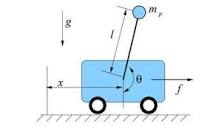
\includegraphics[scale = 0.8, center]{PS3/fig/cartpole.jpeg}

\begin{enumerate}[label=(\alph*)]
    \item What would the optimal feedback control, $a^*$, be at $x_0$ if we are are using LQR-Control at the goal with $K = [1,4,10,-10]$.
    \item Assume that sometime later we have now moved to the state $[0.1,\frac{7\pi}{8},-1,1]^T$. Now what would the optimal feedback control be?
    \item Assume the controller from part (b) agressively overshot the stable upright point and used a large amount of control input. How might you adjust the controller to mitigate that error?
\end{enumerate}

\textbf{Solution 2:}
\begin{enumerate}[label=(\alph*)]
    \item % TODO: Your solution to Problem 2a
    \item % TODO: Your solution to Problem 2b
    \item % TODO: Your solution to Problem 2c
\end{enumerate}

%%%%%%%%%%%%%%%%%%%%%%%%%%%%%%%%%%%%%%%%%%%%%%%%%%%%%%%%%%%%%%%%%%%%%%%%%%%%%%%%%%%%%%%%%%%%%%%%
\clearpage
\textbf{Problem 3: Filtering (7 Points + 2 Bonus)}\\\\
For this problem, you will be playing a typing simulation. Let random variable $E$ represent the observed key press, and $X$ represent the hidden (intended) key press. We have a language with 4 letters (A, B, C, D), and a keyboard arranged as a circle.

\begin{table}[htb]
\centering
    \begin{tabular}{|c|c|}
      \hline
        A & B \\\hline
        C & D \\\hline
    \end{tabular}
\end{table}

At any time, the probability of hitting the intended key is 50\%, and the probability of hitting the neighboring keys is 25\%. For example, $P(E | X = \mathrm{B})$:
\begin{table}[htb]
\centering
    \begin{tabular}{|c|c|}
      \hline
        0.25 & 0.5 \\\hline
        0 & 0.25 \\\hline
    \end{tabular}
\end{table}

In the rest of this problem we will construct and solve for the probabilities of different things occurring using a filtering model over the belief state. Consider the following transition model for $P(X' | X)$:
    \begin{table}[!htb]
    \centering
        \begin{tabular}{|c|c|c|c|c|}
          \hline
             & A' & B' & C' & D' \\\hline
            Begin & 1 & 0 & 0 & 0 \\\hline
            A & 0.5 & 0.5 & 0 & 0 \\\hline
            B & 0 & 0.5 & 0.5 & 0 \\\hline
            C & 0.5 & 0 & 0 & 0.5 \\\hline
            D & 0.25 & 0.25 & 0.25 & 0.25 \\\hline
        \end{tabular}
    \end{table}

\begin{enumerate}[label=(\alph*)]
    \item What is the probability of the sequence of letters ``A B B C D''? 
    
    \item What is the probability of the sequence of letters ``A A B A D''?
    
    \item What is $P(X_3=x | X_1 = \mathrm{A}, X_2 = \mathrm{B})$ for all $x$?
    
    \item Finally we consider the full filtering problem in which we compute $P(X_n | E_1, \ldots, E_n)$. Let ``A B B C D'' be the sequence of observed key strokes. What is the current belief state of the model? We will break this problem down into a few steps. 

    \begin{enumerate}[label=(\roman*)]
        \item First lets assume that for time $n=1$, $B(X_1 = A) = 1$, as our model begins in state A. Compute $P(X_2 = x | E_1, \ldots, E_n)$ where $E$ is defined as above (aka $E_1 = A$, $E_2 = B \dots$).

        Hint: Use both a motion and sensor model to propagate the belief state through time and then update it for the evidence observed! $P(X_n | E_1, ..., E_n) \propto P(E_n|X_n)\sum_{x_{n-1}}P(X_n|x_{n-1})B(x_{n-1})$
        
        \item Continue filtering and compute $P(X_3 = x | E_1, \ldots, E_n)$

        \item For 2 Bonus Points continue filtering and compute \\$P(X_4 = x | E_1, \ldots, E_n)$
    \end{enumerate}

    Note: if you would like to check your answer you can keep going and compute $P(X_5 = x | E_1, \ldots, E_n)$ which should be [0, 0.04, 0, 0.96].
    
\end{enumerate}

\textbf{Solution 3:}
\begin{enumerate}[label=(\alph*)]
    \item % TODO: Your solution to Problem 3a
    \item % TODO: Your solution to Problem 3b
    \item % TODO: Your solution to Problem 3c
    \item \begin{enumerate}[label=(\roman*)]
            \item % TODO: Your solution to Problem 3di
            \item % TODO: Your solution to Problem 3dii
            \item % TODO: Your solution to Problem 3diii
          \end{enumerate}
\end{enumerate}

%%%%%%%%%%%%%%%%%%%%%%%%%%%%%%%%%%%%%%%%%%%%%%%%%%%%%%%%%%%%%%%%%%%%%%%%%%%%%%%%%%%%%%%%%%%%%%%%
\clearpage
\textbf{Problem 4: Computer Vision (10 Points)}\\
\begin{enumerate}[label=(\alph*)]
    \item Assume you have a grayscale input image of a cat with the following pixel values:
        \\ \\
        \begin{tabular}{|c|c|c|c|}
            \hline
            22 & 84 & 1 & 13\\ 
            \hline
            87 & 7 & 144  & 89\\  
            \hline
            222 & 11 & 12 & 144 \\
            \hline
            0 & 95 & 45 & 230 \\
            \hline
        \end{tabular}\\\\
        Also assume you have the following filter:\\\\
        \begin{tabular}{|c|c|c|}
            \hline
            -1 & 1 & 1 \\ 
            \hline
            -2 & 0 & 1\\  
            \hline
            3 & -1 & 0\\
            \hline
        \end{tabular}
        \begin{enumerate}[label=(\roman*)]
            \item What is the size of the output feature map assuming no use of padding or overlap over the edges of the image?
            \item What would the resulting feature map values be?
        \end{enumerate}

    \item Would you classify this image as a dog assume the feature map is passed into an MLP layer using sigmoid as the activation function, assuming the feature map is processed in row major order, neuron weights of [-0.1, -0.2, 0.1, 0.2], a neuron bias of [3.0], and a threshold of $p=0.5$?
    \begin{enumerate}[label=(\roman*)]
        \item What is the output of the MLP?
        \item Would that output be classified as a dog?
    \end{enumerate}
    
    \item True or False and explain in 1-3 sentences:
        \begin{enumerate}[label=(\roman*)]
            \item The Gaussian filter helps smooth out images and is NOT helpful for finding features such as edges.
            \item The derivative filter helps smooth out images and is NOT helpful for finding features such as edges.
            \item The RANSAC algorithm is always able to find a model that fits all of the datapoints.
            \item Convolutional Neural Networks can only fit data to predict one class at a time.
        \end{enumerate}
    
\end{enumerate}

\textbf{Solution 4:}
\begin{enumerate}[label=(\alph*)]
    \item \begin{enumerate}[label=(\roman*)]
            \item % TODO: Your solution to Problem 4ai
            \item % TODO: Your solution to Problem 4aii
          \end{enumerate}    
    
    \item \begin{enumerate}[label=(\roman*)]
            \item % TODO: Your solution to Problem 4bi
            \item % TODO: Your solution to Problem 4bii
        \end{enumerate}
    
    \item \begin{enumerate}[label=(\roman*)]
            \item % TODO: Your solution to Problem 4ci
            \item % TODO: Your solution to Problem 4cii
            \item % TODO: Your solution to Problem 4ciii
            \item % TODO: Your solution to Problem 4civ
        \end{enumerate}
\end{enumerate}


%%%%%%%%%%%%%%%%%%%%%%%%%%%%%%%%%%%%%%%%%%%%%%%%%%%%%%%%%%%%%%%%%%%%%%%%%%%%%%%%%%%%%%%%%%%%%%%%
\clearpage
\textbf{Problem 5: Computer Vision Experiment (3 Points)}\\

A software based question in the written?!? What!?! Well it turns out this is more of an experiment with an online interface than a true coding questions so its best if you upload a screenshot to show that you did it!

Go to \url{https://teachablemachine.withgoogle.com/}. 

There you will find a whole host of documentation and videos on how to get started using their free platform for training simple neural network models. It turns out that while training a large, sophisticated model can take a long time, training a simple, small model is a breeze!

Click on \texttt{Get Started $->$ Image Project $->$ Standard Image Model}. You should arrive at a screen that looks something like the below:

\begin{center}
    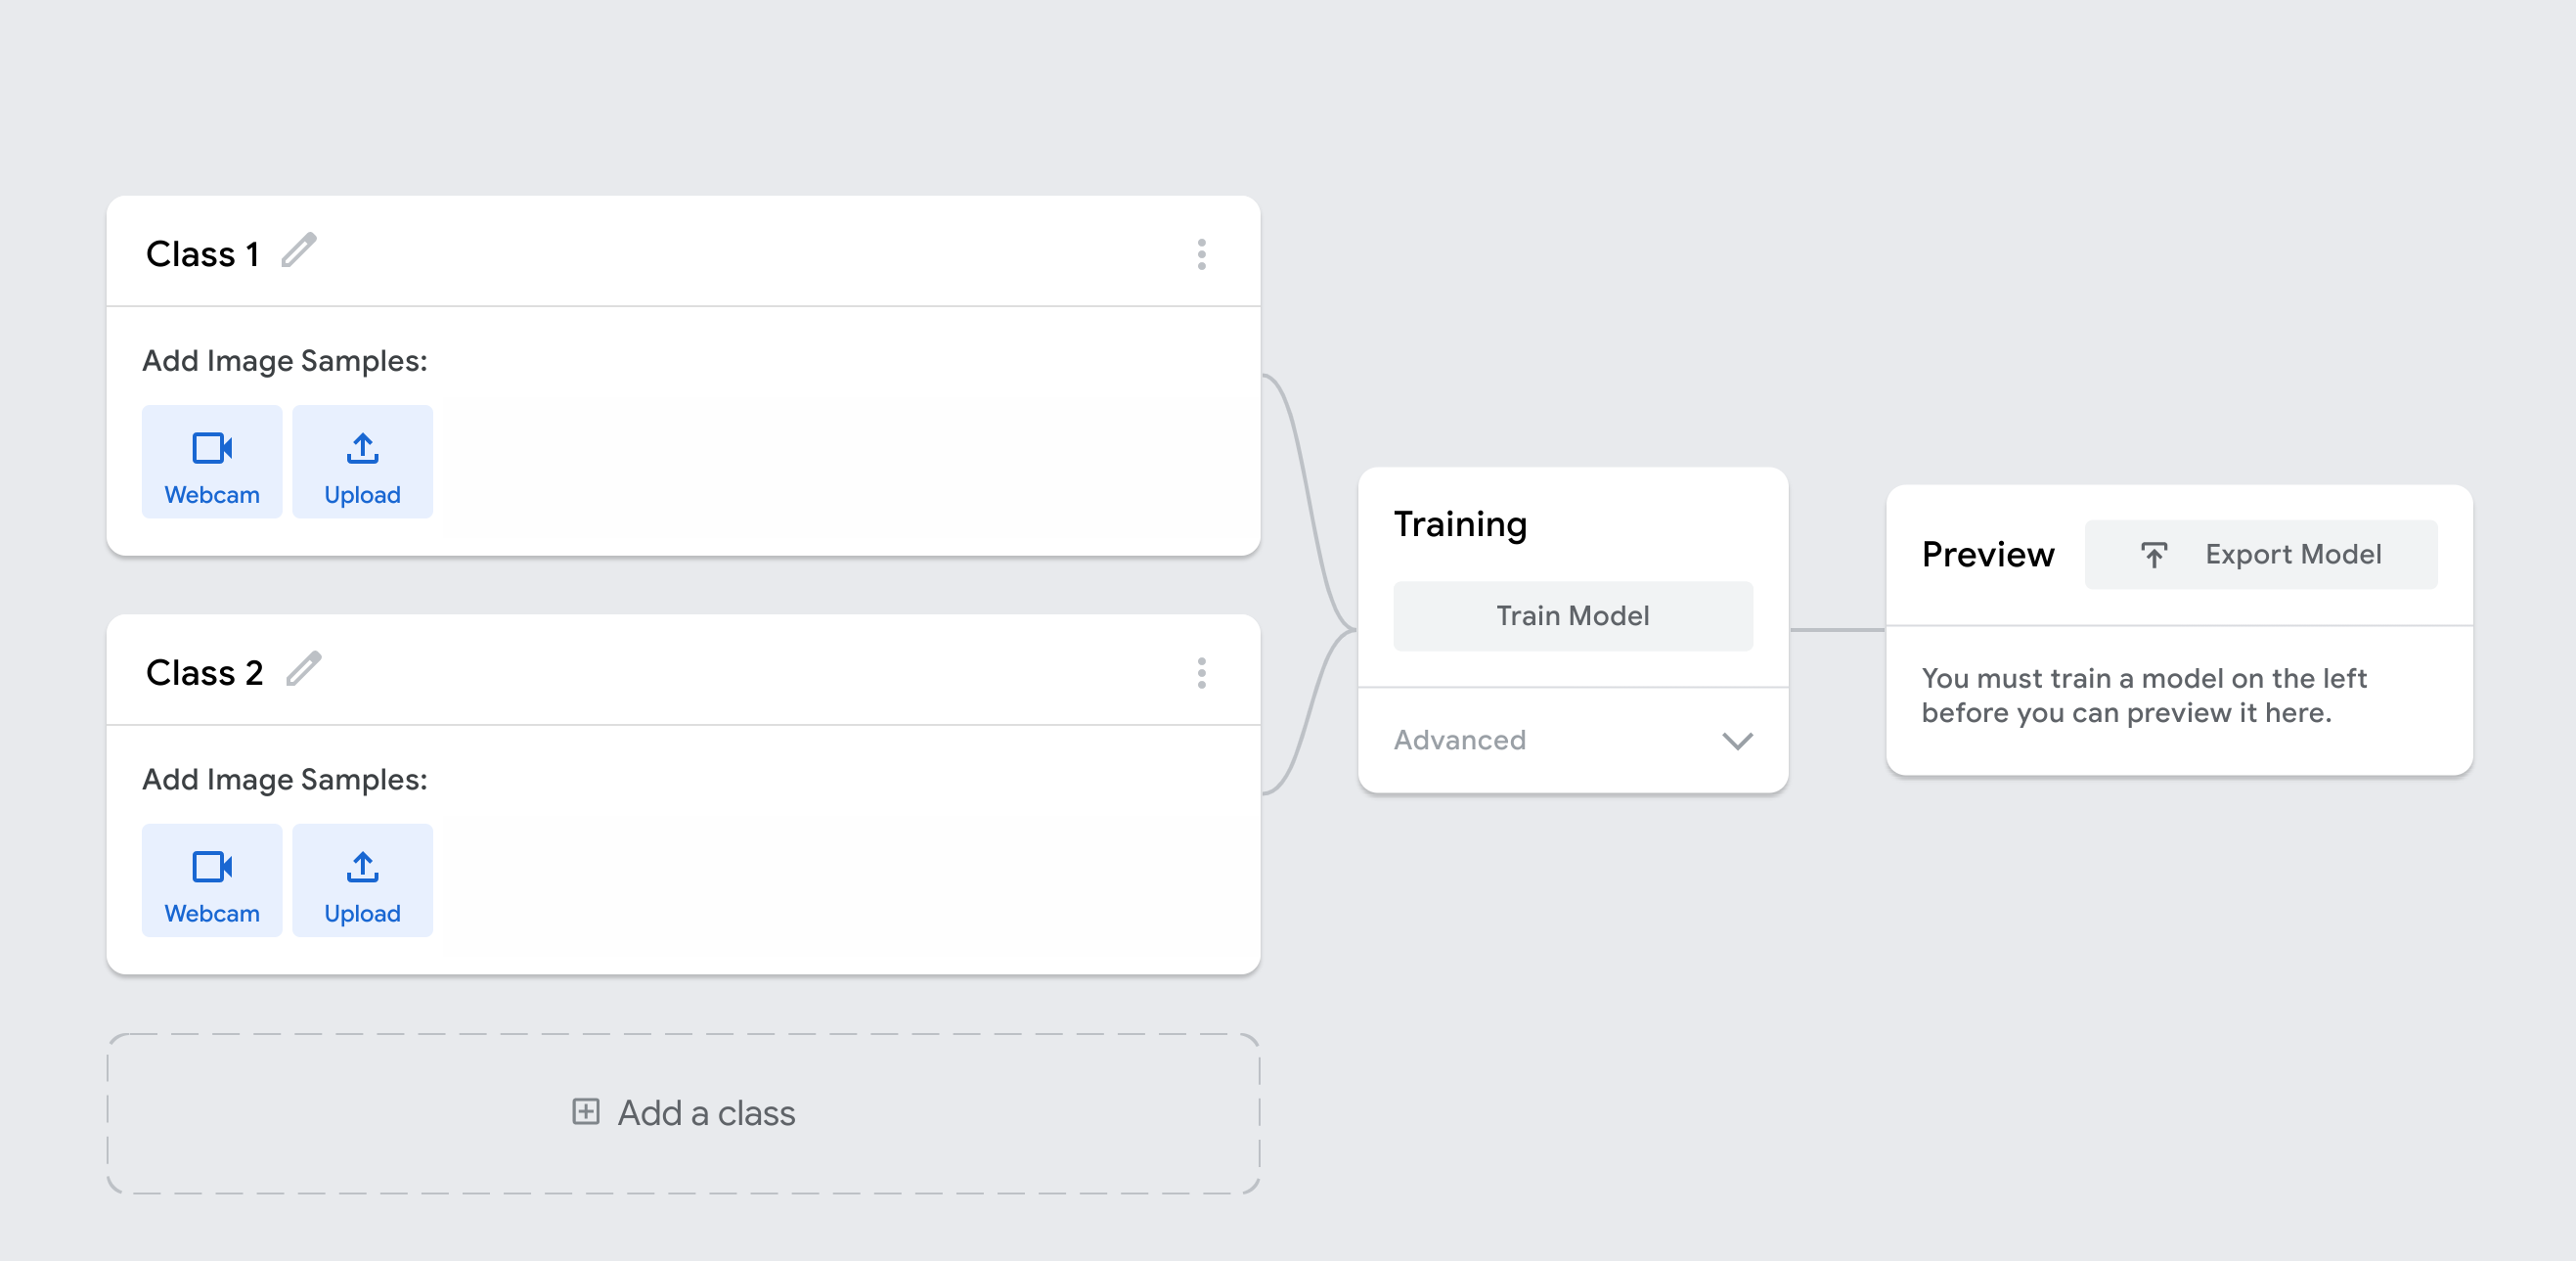
\includegraphics[width=0.7\textwidth]{PS4/figs/screenshot1.png}    
\end{center}

You'll want to pick between 2-5 objects that you want to train a model to differentiate between (you can add more classes by clicking \texttt{Add a class} at the bottom). You can name the classes and the use your webcam or upload pictures of the classes. Try to pick objects that look distinctively different for at least a few of the classes (and then feel free to throw in one hard one if you'd like). Make sure you upload / take 30-50 images of each class.

Then click \texttt{Train Model} which will likely take a surprisingly short amount of time! Then you can preview your results. Please submit a screenshot of the final trained model running on one of your classes like the image below of me!

\begin{center}
    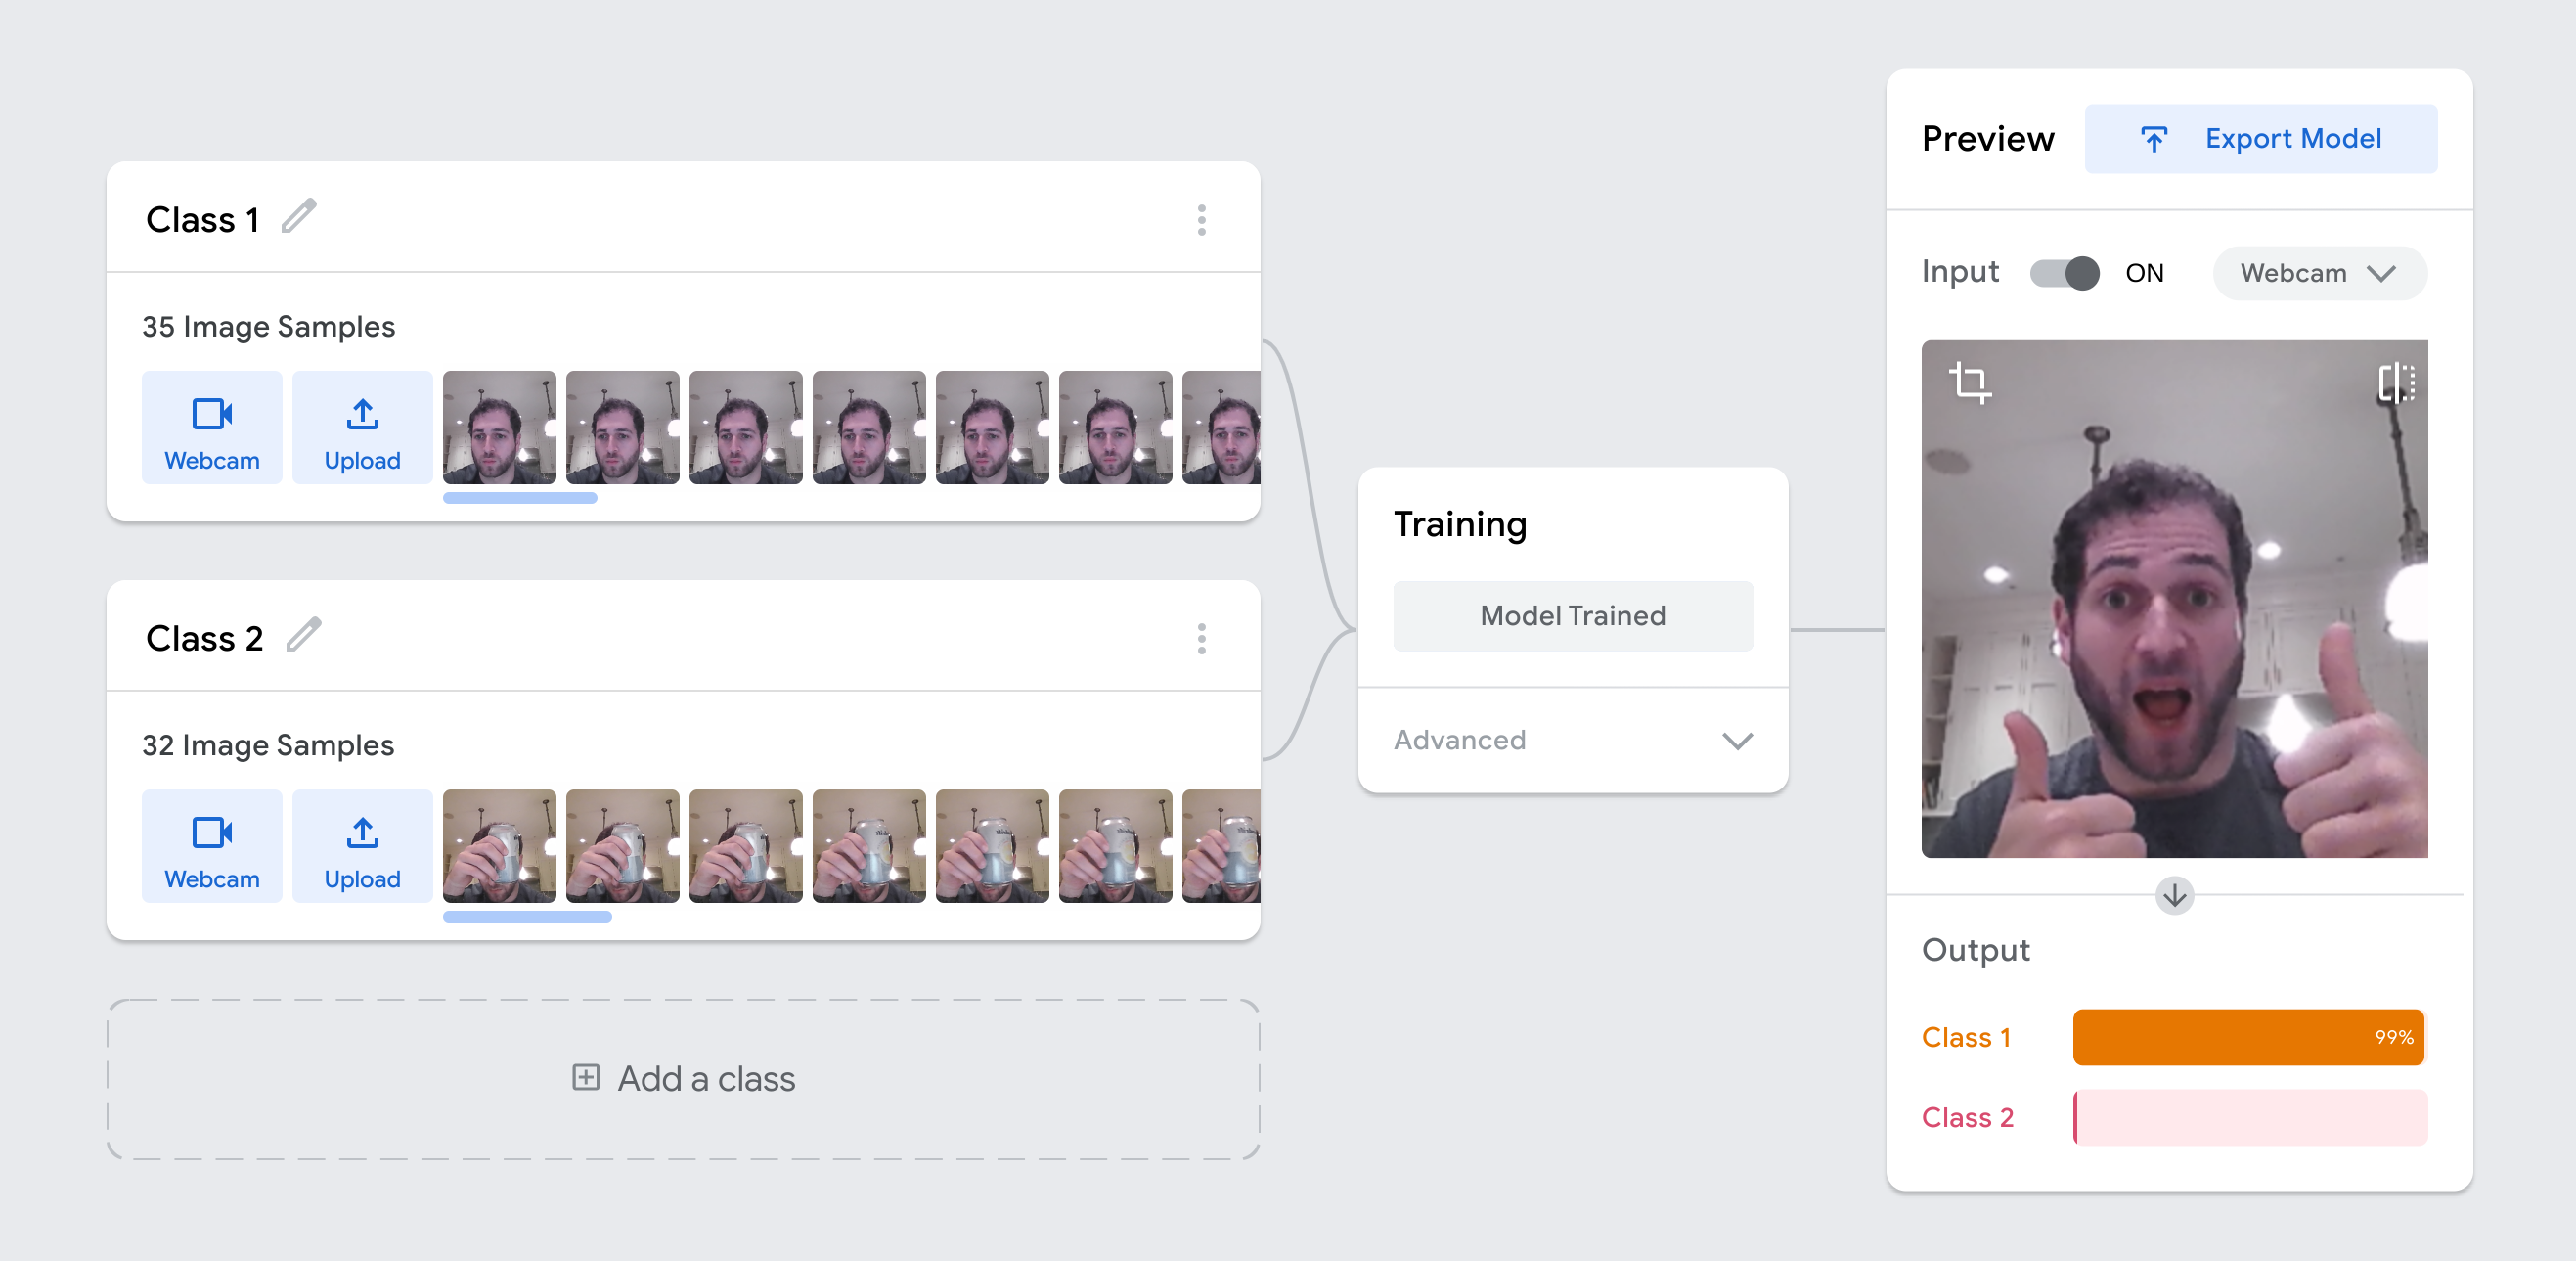
\includegraphics[width=0.7\textwidth]{PS4/figs/screenshot2.png}    
\end{center}

\textbf{Solution 5:}
% TODO: Your solution to Problem 5

\end{document}